\section{Estimación de Pose 3D}

En la sección \ref{sec:taxonomy}, previamente mencionamos que la estimación de pose puede hacerse
en dos etapas. La primer etapa encargada de predecir las poses en 2 dimensiones y la segunda en
realizar la predicción a 3 dimensiones a partir de los resultados de la etapa anterior. Este esquema
de predicción y entrenamiento fue uno de los primeros propuestos por J. Martinez
\cite{DBLP:journals/corr/MartinezHRL17}. La tarea de estimación de pose 2D está relativamente madura
con resultados bastante precisos, así que suena prudente aprovechar estos modelos ya existentes para
resolver un primera parte del problema. Así, Martinez entrena un nuevo modelo que utiliza esta
información para generar la poses en un dimensión más alta, dejando los problemas como lidiar con las
escenas de fondo, iluminación, color y texturas de las ropas, color de piel o diversas imperfecciones
de las imágenes, en la primer etapa.

\begin{figure}[!ht]
    \centering
    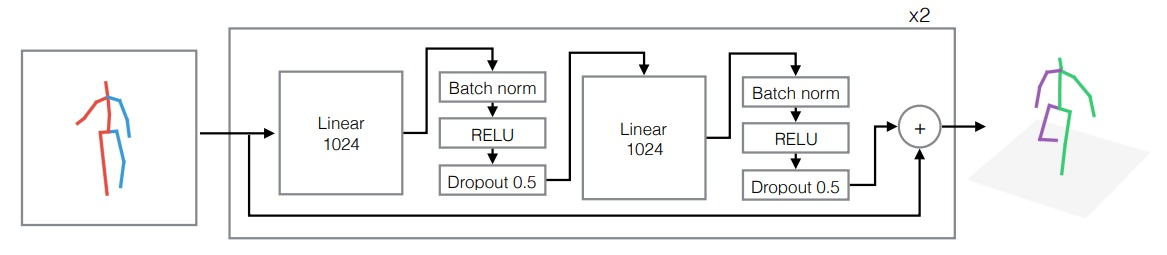
\includegraphics[width=.9\textwidth]{Chapters/3. Trans-HPE/img/martinez_model.jpeg}
    \caption[2D a 3D model]{Modelo usado por J. Martinez \cite{DBLP:journals/corr/MartinezHRL17}
    basado en una simple red neuronal multicapa usando batch normalization, dropout, Rectified
    Linear Units y residual connections.}
\label{fig:model_martinez}
\end{figure}

En la figura \ref{fig:model_martinez} se muestra el modelo usado por J. Martinez. Los datos de entrada
son las posiciones de las articulaciones del cuerpo humano, estos son incrementados de dimensión a
1024 usando la primer capa lineal, posteriormente pasa a un proceso de normalización por lotes
y son activados con una función \textit{RELU} con dropout de 50 por ciento. La salida de este modelo
es proyectada para tener una dimensión de $3n$ con $n$ como el número de articulaciones, representando
puntos en un espacio de 3 dimensiones.

Siguiendo la misma estrategia \citeauthor{DBLP:journals/corr/abs-2009-00348}
\cite{DBLP:journals/corr/abs-2009-00348} utiliza una arquitectura
basada en el Transformer presentado por \citeauthor{Vaswani} \cite{Vaswani}. Un Transformer con capas
ocultas de dimensión 512, 8 cabeza de multi-atención y bloques codificadores como se observa en la
figura \ref{fig:Liftformerfig}.

\begin{figure}[!ht]
    \centering
    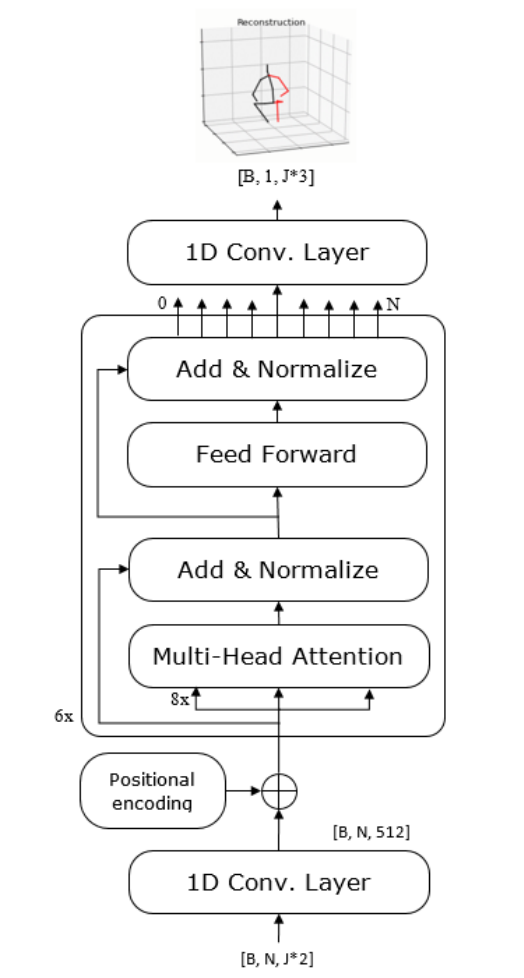
\includegraphics[width=.4\textwidth]{Chapters/3. Trans-HPE/img/poseTrans.png}
    \caption[Liftformer]{Liftformer
    \cite{DBLP:journals/corr/abs-2009-00348}, modelo basado en la parte codificadora del un Transformer.
    Predice los puntos de articulación 3D a partir de una secuencia de puntos 2D.}
\label{fig:Liftformerfig}
\end{figure}

Liftformer solo implementa la parte codificadora del modelo de
Transformer sin ningún otro cambio a este. Durante el entrenamiento utiliza como entrada una secuencia
de coordenadas representando las puntos de articulaciones en dos dimenciones. La primer mitad corresponde
a información del pasado y la segunda mitad a información del futuro generando una predicción de pose
3D correspondiente al centro de la secuencia de entrada.

Al inicio del modelo la información es reproyectada de un espacio de $[N, 34]$ a $[N, 512]$ a través
de una capa Convolucional de una dimención. En este misma etapa es inyectada la información temporal
a usando \textit{temporal embeddings}. De manera similar y dado que no es usado un decodificador
el modelo elige el token correspondiente a la mitad de los datos de entrada repoyectándolo a dimenciones
$[1, 51]$. Las 17 articulaciones y en coordenadas x, y, z estarán representadas por este vector de 51
elementos.

Proyecto enfocado solo en Estimación de pose 2D HPE y 3D HPE considerando un solo objetivo SPPE

Para el primer caso solo martinez solo se enfoca en el segundo stage de la estimación de pose
no se usa un modelo end-to-end sino que aprovecha los modelos ya creados para estimación de pose
en 2d y a

Explicar las arquitecturas usadadas
- la de martinez
- La del transformer
- La que funciona

\section{Modificación a transformers - Usando cabezas de Atención flexibles}

\section{Evaluación y comparativas}
